\StartPlate{V17}{Clifford dimensions keep the radical and orbit factors}{An abstract packet count must match an actual restriction problem.}
\begin{center}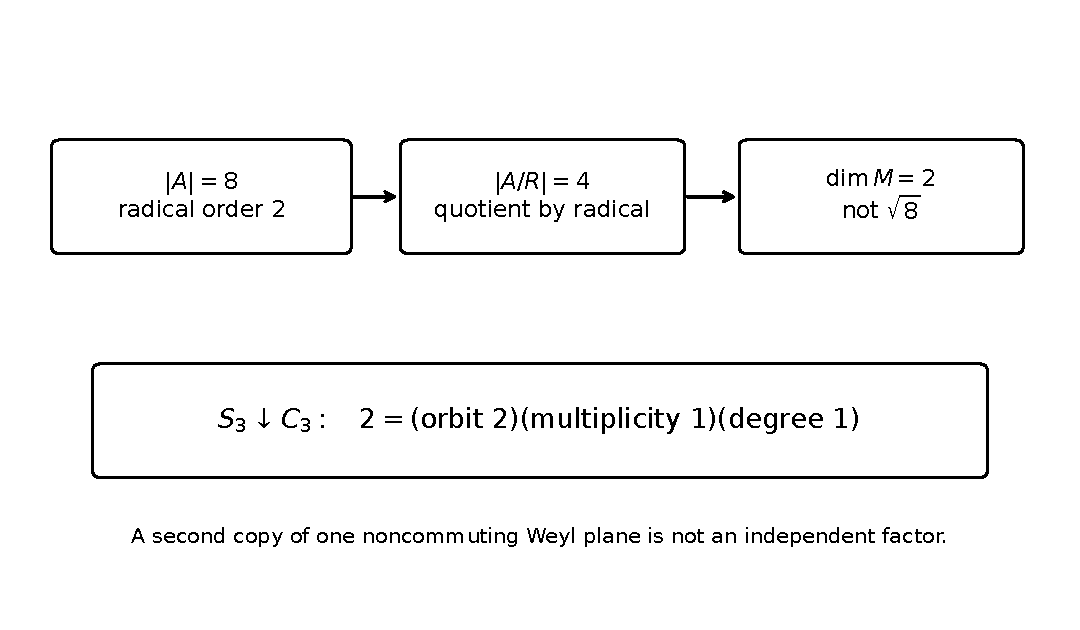
\includegraphics[width=\linewidth]{figures/V17.pdf}\end{center}
For a finite abelian projective quotient $A$, let $R$ be the radical of its commutator pairing. An irreducible projective multiplicity has degree
\[
(\dim M)^2=|A/R|.
\]
The first example uses $A=\F_2^3$, with the standard symplectic pairing on the first two coordinates and the third coordinate radical. Thus $|A|=8$, $|R|=2$, and $\dim M=2$. Suppressing the radical would incorrectly produce $\sqrt8$.

The second example retains the inertia orbit. The two-dimensional irreducible of $S_3$ restricts to two distinct nontrivial characters of $C_3$. Each multiplicity is one, but the orbit has size two. Along a genuine compatible chain, every orbit factor and every projective multiplicity must be retained.

Independent commuting projective factors on the same carrier multiply their degrees. Representing one Weyl plane twice on the same space does not create independent commuting factors. The finite matrix checks include the $S_3$ relations, while the general restriction argument remains in the paper.
\vfill\PlateSource{Exact projective and orbit models}{Part II, Section 15}{41}
